%% Label Bias and Environmental Datashift
\chapter{Label Bias and Environmental Datashift}
Bias is the result of inadequate data where a certain group or class is favoured over another/others hence creating an overrepresentation \cite{Jiang}\cite{saria2019tutorial}.
ML models trained using such datasets will acquire these underlying biases hence making incorrect predictions.

The following mathematical framework developed by researches at Google can be used as a representation to undestand bias in data \cite{Jiang}

\begin{figure}[h]
    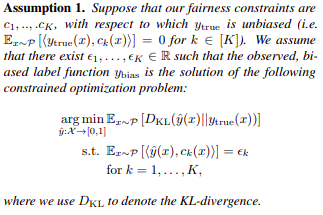
\includegraphics[scale =0.8]{Assumption.png}
    \centering
    \caption{Bias Assumption \cite{Jiang}}
    \label{fig:Assumption}
\end{figure}

In figure \ref{fig:Assumption}, the assumption is that $y_{bias}$ is the label which is closest to $y_{true}$ and achieves a measure of bias.
In cases where data has been manually manipulated by human input, either consciously or subconsciously, this is deemed to be a reasonable assumption.
The contiguity to $y_{true}$ is given by the KL-divergance, which is used to establish the notion of accurate labeling. 
The Proposition in figure \ref{fig:Proposition} is derived from the KL-divergence. (For complete proof of proposition, see \cite{Jiang})

\begin{figure}[h]
    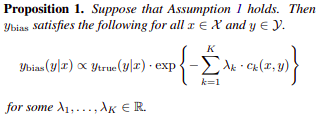
\includegraphics[scale =0.8]{Prop.png}
    \centering
    \caption{Bias Proposition \cite{Jiang}}
    \label{fig:Proposition}
\end{figure}

Now that $y_{bias}$ is represented in terms of $y_{true}$, we can infer $y_{true}$ in terms of $y_{bias}$ as represented in Figure \ref{fig:Corollary}.

\begin{figure}[h]
    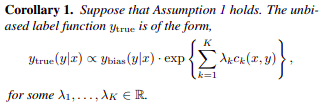
\includegraphics[scale =0.8]{corollary.png}
    \centering
    \caption{Bias Corollary \cite{Jiang}}
    \label{fig:Corollary}
\end{figure}

There may be situations where performance issues may not be apparent during training stages. 
They instead appear post-deployment where training and deployment datasets can have irregularities. 
This is known as Environmental Datashift \cite{saria2019tutorial}. 
This calls into question whether the ML model is robust enough to generalise well to new samples beyond training, or whether it tends to over-generalise to the training dataset thus resulting in unreliability in the real world.
\hl{maths}

\section{Dataset \& Preprocessing}
The predictive maintenance dataset will be used again to classify failures of an ioT gadget.
During one week, maintenance data was collected from six devices every hour for 168 hrs.
Therefore, this data set contains 1008 rows of data. 
Each cycle of data reading contains the following measurements: 

\begin{table}[H]
    \begin{center}
        \caption{Measurements Dataset} 
        \begin{tabular}{ l|l } 
         \toprule
         \textbf{Measurement} & \textbf{Description} \\  [0.5ex] 
         \midrule
         \textbf{Measurement Time} & Time \\
         \textbf{Gadget ID} & Device number \\
         \textbf{Vibration x sensor} & Horizontal vibration \\ 
         \textbf{Vibration y sensor} & Vertical vibration \\ 
         \textbf{Pressure sensor} & Hose pressure \\
         \textbf{Temperature sensor} & Internal temperature \\
         \bottomrule
        \end{tabular}
    \end{center}
\end{table}

The failures dataset contains the precise times each gadget failed. 
During the course of the week, 105 failures were recorded. 
The two datasets were combined and additional labels were added (\ref{table:labels}) for use in training and prediction.
The model was trained using \textit{'Vibration y'}, \textit{'Temperature 6hr Std'}, 
and \textit{'Pressure 6hr Mean'} as feature labels, and predictions were tested using class label, \textit{'Fail in 1hr'},
where positive classification of device failure occurs when the time remaining to device failure is less than one hour.

\begin{table}[H]
    \begin{center}
        \caption{Maniupulated data labels}
        \label{table:labels} 
        \begin{tabular}{l|l}
            \toprule
            \textbf{Labels} & \textbf{Description} \\ [0.5ex]
            \midrule
            \textbf{Temperature 6hr Std} & Standard Deviation of last 6 measurements \\
            \textbf{Pressure 6hr Mean} & Average of last 6 measurements \\
            \textbf{Fail in 1hr} & If failure will occur within the next hour \\
            \bottomrule
        \end{tabular}
    \end{center}
\end{table}

The complete dataset was then split 70-30\% for training and testing respectively. 
In addition, the train dataset was split into two further datasets, DF1 and DF2. 
DF1 contained all data from devices with 'Gadget ID' 1,2 and 3 while DF2 contained all data from devices with 'Gadget ID' 3,4 and 5.
Concsequently, the test dataset was also split into 'Sample 1' and 'Sample 2' in the same manner as DF1 and DF2.

\begin{table}[H]
    \begin{center}
        \caption{Training and Testing Datasets}
        \label{table:datasets} 
        \begin{tabular}{l|l|l}
            \toprule
            \textbf{Dataset} & \textbf{Size} &\textbf{Description} \\ [0.5ex]
            \midrule
            \textbf{Full Train} &685& 70\% of the complete dataset. Used for training model \\
            \textbf{Full Test} &293& 30\% of the complete dataset. Used for testing model \\
            \textbf{DF1} &339& All samples from \textbf{Full Train} with Gadget ID 1,2 \& 3 only \\
            \textbf{DF2} &346& All samples from \textbf{Full Train} with Gadget ID 4,5 \& 6 only \\
            \textbf{Sample 1} &150& All samples from \textbf{Full Test} with Gadget ID 1,2 \& 3 only \\
            \textbf{Sample 2} &145& All samples from \textbf{Full Test} with Gadget ID 4,5 \& 6 only \\
            \bottomrule
        \end{tabular}
    \end{center}
\end{table}

\section{Results}
\begin{table}[H]
    \begin{center}
        \caption{PDM Label Bias and Environmental Datashift Evaluation Results}
        \label{table:Bias}
        \begin{tabular}{lccccccc}
            \toprule
            \multicolumn{1}{c}{\textbf{Metric}} & \multicolumn{7}{c}{\textbf{Datasets}}                                                                                                                                                                                                      \\ \midrule
            \multicolumn{1}{l}{}      & \multicolumn{1}{c|}{Full Train} & \multicolumn{3}{c|}{DF1}                                                                       & \multicolumn{3}{c}{DF2}                                                                       \\ \cline{2-8} 
            \multicolumn{1}{l}{}      & \multicolumn{1}{l|}{Full Test}  & \multicolumn{1}{l|}{Full Test} & \multicolumn{1}{l|}{Sample 1} & \multicolumn{1}{l|}{DF2} & \multicolumn{1}{l|}{Full Test} & \multicolumn{1}{l|}{Sample 2} & \multicolumn{1}{l}{DF1} \\ 
            \midrule
            \textbf{Accuracy} & 0.71 &0.717 &0.774 &0.731 &0.71 &0.789 &0.673\\
            \textbf{Precision} &0.9 &0.90 &0.90 &0.92 &0.90 &0.93 &0.91\\
            \textbf{Recall} &0.71 &0.72 &0.77 &0.73 &0.71 &0.79 &0.67\\
            \textbf{F1 Score} &0.77 &0.77 &0.81 &0.78 &0.77 &0.83 &0.75\\
            % \midrule
            % \bottomrule
        \end{tabular}
    \end{center}
\end{table}

\begin{figure}[H]
    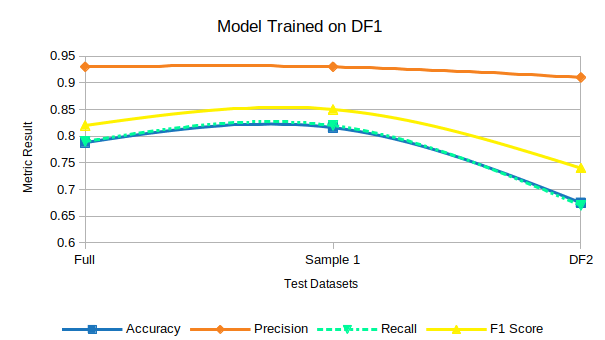
\includegraphics[scale =0.8]{Bias_DF1.png}
    \centering
    \caption{Test Datasets on DF1 metrios}
    \label{fig:DF1}
\end{figure}
\begin{figure}[H]
    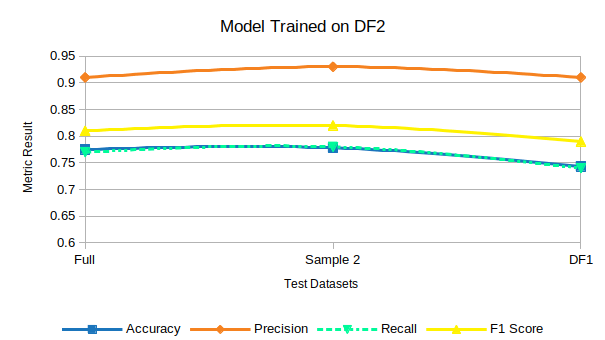
\includegraphics[scale =0.8]{Bias_DF2.png}
    \centering
    \caption{Test Datasets on DF2 metrios}
    \label{fig:DF2}
\end{figure}

\hl{Consider noise in dataset due to uneccassry labels}

Datashift:
\hl{The issue is that modelers typically assume that training data
is representative of the target population or environment where
the model will be deployed} \cite{saria2019tutorial}

\section{Discussion}
